\chapter{Aplicaciones}

Una de las principales y comunes aplicaciones de las ED en ingeniería son en el uso y calculo de voltaje o corriente en los Circuitos RLC:

\begin{center}
  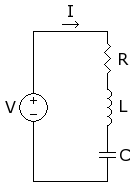
\includegraphics[scale=0.5]{imgsAux/rlc.png}
\end{center}

Dos principios físicos que rigen a los Circuitos RLC en serie son:

\begin{enumerate}
  \item La conservación de la Carga Electrica \(\displaystyle(Q)\)
  \item La conservación de la Energía
\end{enumerate}

Estas leyes de la conservación para Circuitos Electricos estan dados por la función formulada por G. Kirchhoff en 1859 y se llaman Leyes de Kirchhoff, las cuales no dicen:

\begin{enumerate}
  \item La corriente \(\displaystyle I\) que circula a traves de cada uno de los elementos en serie debe ser la misma.
  \item La suma algebraica de los cambios instantáneos de potencial (Caídas de voltaje) alrededor de un Circuito cerrado debe ser cero y los voltajes de cada elemento son dados por:

  \begin{enumerate}
    \item Resistencia (R):

    \begin{itemize}
      \item Ley de Ohm
      \item \(\displaystyle V_{R}=IR \)
      \item \(\displaystyle V_{R}\) Caída de voltaje (Volts: V)
      \item \(\displaystyle I\) Intensidad de Corriente (Amperes: A)
      \item \(\displaystyle R\) Resistencia (Ohms: \(\displaystyle\Omega\))
    \end{itemize}

    \item Inductor (Bobina) (L):
    \begin{itemize}
      \item Por las leyes de Faraday y la Ley de Lenz:
      \item \(\displaystyle V_{L}=L\frac{dI}{dt} \)
      \item \(\displaystyle V_{L}\) Voltaje (V)
      \item \(\displaystyle L\) Bobina o inductor (Henrys:hy)
      \item \(\displaystyle I\) Intensidad de Corriente (A)
    \end{itemize}

    \item Capacitor (C):
    \begin{itemize}
      \item \(\displaystyle V_{C}=\frac{Q}{C}\)
      \item \(\displaystyle V_{C}\) Voltaje (V)
      \item \(\displaystyle C\) Capacitor (Farads:Fd)
      \item \(\displaystyle Q\) Carga (Coulombs:C)
    \end{itemize}
  \end{enumerate}
\end{enumerate}

La fuerza electromotriz proporciona voltaje o energía potencial al Circuito. Si denotamos a \(\displaystyle V\) como \(\displaystyle E(t)\) y lo llamamos al voltaje  aplicado al tiempo \(\displaystyle t\), entonces la Ley de Kirchhoff de conservación de la energía es:

\begin{equation*}
    \begin{gathered}
        E(t)=V_{R}+V_{L}+V_{C}
    \end{gathered}
\end{equation*}

Sustituyendo esta formula con las definiciones de voltaje previamente explicadas, tendremos:

\begin{equation*}
    \begin{gathered}
        E(t)=IR+L\frac{dI}{dt}+\frac{1}{C}Q
    \end{gathered}
\end{equation*}

Remarcando que \(\displaystyle I=\frac{dQ}{dt}\), entonces tendremos la ED:

\begin{equation*}
    \begin{gathered}
        E(t)=L\frac{d^{2}Q}{dt^{2}}+R\frac{dQ}{dt}+\frac{1}{C}Q\;\;ED\;de\;2^{do}\;orden
    \end{gathered}
\end{equation*}

Para este caso de primer orden pensaremos en circuitos RL o RC, quedando ED de primer orden.

\section{RC}
Para este caso la ED sería:
\begin{equation*}
    \begin{gathered}
        R\frac{dQ}{dt}+\frac{1}{C}Q=E(t)
    \end{gathered}
\end{equation*}

Normalizando:

\begin{equation*}
    \begin{gathered}
        \dot{Q}+\frac{1}{RC}Q=\frac{E(t)}{R}
    \end{gathered}
\end{equation*}

\section{RL}

Para este caso la ED sería:

\begin{equation*}
    \begin{gathered}
        L\frac{dI}{dt}+RI=E(t)
    \end{gathered}
\end{equation*}

Normalizando:

\begin{equation*}
    \begin{gathered}
        \dot{I}+\frac{R}{L}I=\frac{E(t)}{L}
    \end{gathered}
\end{equation*}

\textit{Nota: Resolver como los ejercicios normales, solo cuidar las unidades con las que se trabajan}\\

\textbf{Ejercicios propuestos}

\begin{enumerate}
  \item Considere un Circuito RC con \(\displaystyle R=120\Omega\) y \(\displaystyle C=\frac{1}{1200}fd\) al tiempo \(\displaystyle t=0\) se conecta una fuente de voltaje constante de \(\displaystyle E(t)=120V\) si inicialmente la carga \(\displaystyle Q=0\), determine como cambia la carga en el capacitor y la corriente del circuito.
  \item Se conecta un resistor \(\displaystyle R=40\Omega\) y un Inductor \(\displaystyle L=0.1hy\), con una fuente de \(\displaystyle E(t)=110V\) si originalmente no hay corriente al \(\displaystyle t=0\) \(\displaystyle I(t=0)=0\) determine la corriente al tiempo \(\displaystyle t\)
\end{enumerate}